\subsection{Motivation}

In order to try to confirm that the game variants had the intended effects on gameplay, we initially generated AI agents to play the games. We would then log the score, velocity, and missile count of each of the agents over the course of multiple runs, and use these results to try to try to quantify the effects of the variations on gameplay.

\subsection{Methodology}

For the purpose of testing the different variations of the game, 4 agents were used:
\begin{itemize}
	\item EmptyController, an agent that performs no actions
	\item RotateAndShoot, an agent that continually turns in a single direction while shooting
	\item MMMCTS, a version of Monte Carlo Tree Search using hand-crafted heuristics that is given 40ms to select an action
	\item MMMCTS2, which is identical to MCTS but with a shorter 20ms computational budget
\end{itemize}

Agents of different complexity were used in order to estimate the difference between the results of skilled versus unskilled players. For this, we consider EmptyController to represent the weakest of players who do not react to what is on the screen. By comparison, we would expect the RotateAndShoot agent to represent a slightly more skilled player who attempts to shoot the enemy ship, but has little strategy or skill. Finally, we would employ the MCTS-based agents to represent skilled players that would do whatever they could to win the game, always planning ahead a short amount into the future. Between the two, we would expect the MCTS agent with a larger computational budget to perform better, as the additional time given to make decisions would allow the agent to build a larger tree of known states, and therefore could plan further into the future.

The MCTS agents used in this assessment were partially based of the winner of the Physical Travelling Salesman Competition\cite{6374161}. The exact implementation for this problem included macro-actions of length 3\footnote{In order to stop the MCTS agents from quickly expending the limited missile count, any macro-actions that would have included firing for each of the three primitive actions instead only fires for the first, with the thrust and turning values being unchanged.}. 

These agents were made to compete in a round-robin tournament for all three game variations over 30 trials. During the tournament, the score, remaining missile count, and velocity of each agent was logged, with the results analysed at the end. Comparisons between like agents (e.g. MMMCTS versus MMMCTS) were not computed in order to save time. Plots of the score and missile count averaged over all runs for each agent can be seen in Figures \ref{fig:data1}, \ref{fig:data2}, and \ref{fig:data3}.

\subsection{Results}

Looking at the performance of the agents, the results are remarkably similar to our expectations. The EmptyController agent always performed the worst, managing the occasional win against agents that were unlucky in hitting many asteroids, and therefore ending with a negative score. The RotateAndShoot agent performed slightly better, more often than not beating the EmptyController agent, but still losing to the MCTS agents. The MCTS agents were dominant compared to the non-MCTS agents, and the one given a larger computational budget ended up usually outperforming the one with the tighter budget.

Looking at the graphs of score-versus-time for each game mode, we can see that the first game variant (including simple asteroids) resulted in the simpler agents ending with a slightly negative score, with this effect being significantly stronger in the second game variant (featuring splitting asteroids). This is inkeeping with what we expected, although the effect is slightly smaller than we had hoped.

Comparison of the average velocity for the MCTS agents for each of the game variations suggests that the two variants including asteroids resulted in the agents moving at a higher average speed. This is as we had expected, and could suggest that in this respect the inclusion of asteroids had the desired impact.

\begin{figure}
	\caption{AI results over the game without asteroids}
	\begin{tabular}{x{7.1em} | x{4.2em} x{4.1em} x{3.1em} x{3.1em}}
		&
			Empty Controller &
			Rotate and Shoot &
			MCTS (20ms) &
			MCTS (40ms) \\ \hline
		Empty Controller &
			-&
			0\% &
			3\% &
			0\% \\
		Rotate and Shoot &
			100\% &
			-&
			3\% &
			3\% \\ 
		MCTS (20ms) &
			97\% &
			97\% &
			-&
			30\% \\
		MCTS (40ms) &
			100\% &
			97\% &
			70\% &
			-\\
	\end{tabular}
	\vspace{1em}
	\caption{AI results over the game with simple asteroids}
	\begin{tabular}{x{7.1em} | x{4.2em} x{4.1em} x{3.1em} x{3.1em}}
		&
			Empty Controller &
			Rotate and Shoot &
			MCTS (20ms) &
			MCTS (40ms) \\ \hline
		Empty Controller &
			-&
			0\% &
			0\% &
			0\% \\
		Rotate and Shoot &
			100\% &
			-&
			20\% &
			6\% \\ 
		MCTS (20ms) &
			100\% &
			80\% &
			-&
			57\% \\
		MCTS (40ms) &
			100\% &
			93\% &
			44\% &
			-\\
	\end{tabular}
	\vspace{1em}
	\caption{AI results over the game with splitting asteroids}
	\begin{tabular}{x{7.1em} | x{4.2em} x{4.1em} x{3.1em} x{3.1em}}
		&
			Empty Controller &
			Rotate and Shoot &
			MCTS (20ms) &
			MCTS (40ms) \\ \hline
		Empty Controller &
			-&
			3\% &
			0\% &	
			0\% \\
		Rotate and Shoot &
			97\% &
			-&
			3\% &
			0\% \\ 
		MCTS (20ms) &
			100\% &
			97\% &
			-&
			30\% \\
		MCTS (40ms) &
			100\% &
			100\% &
			70\% &
			-\\
	\end{tabular}
\end{figure}

\begin{figure*}
	\caption{Average metrics for AI players over the game without asteroids}
	\label{fig:data1}
	\center
	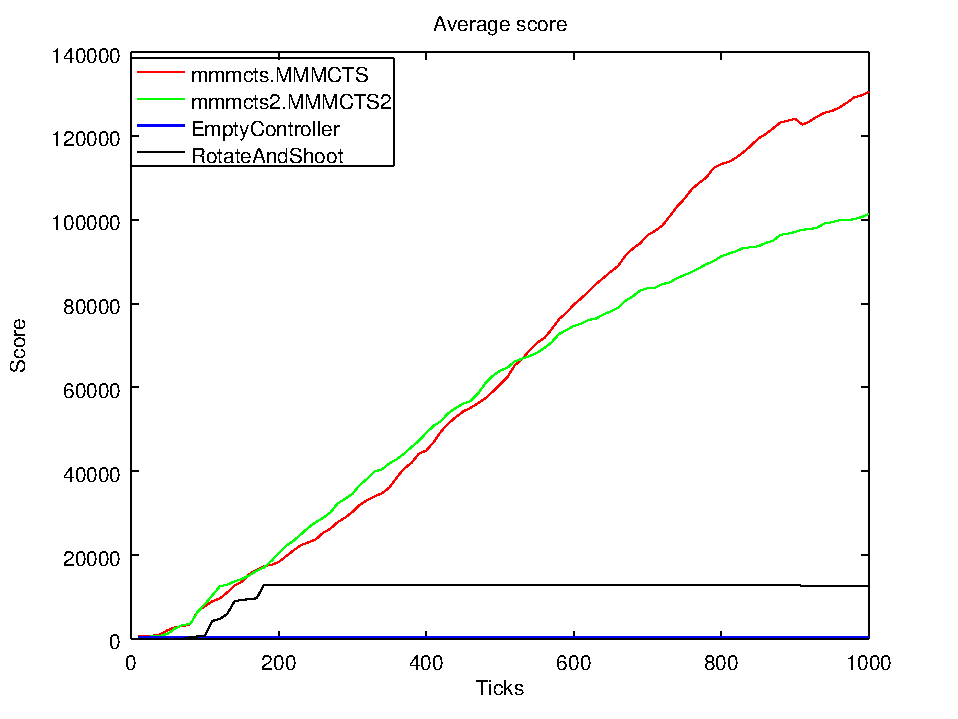
\includegraphics[scale=0.4]{resources/score_2.pdf}
	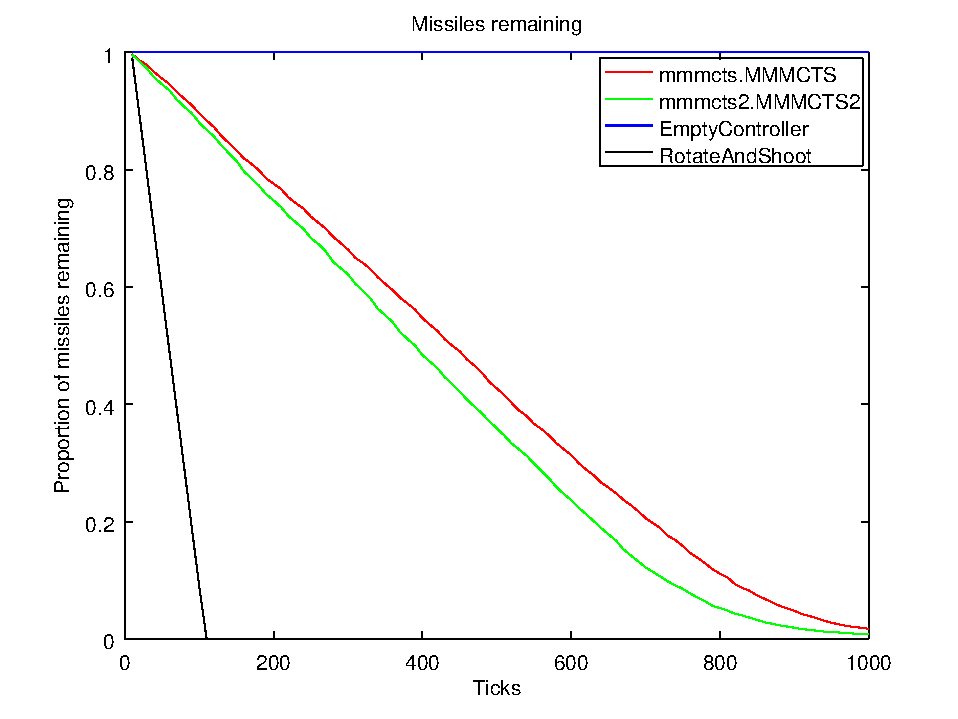
\includegraphics[scale=0.4]{resources/missiles_2.pdf}
\end{figure*}

\begin{figure*}
	\caption{Average metrics for AI players over the game with simple asteroids}
	\label{fig:data2}
	\center
	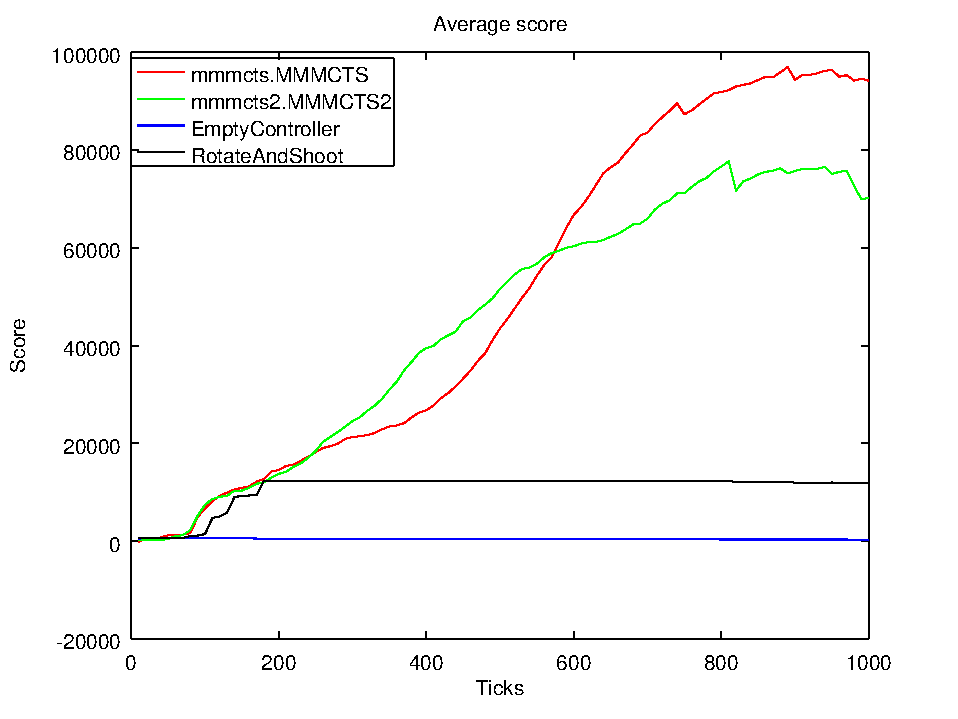
\includegraphics[scale=0.4]{resources/score_1.pdf}
	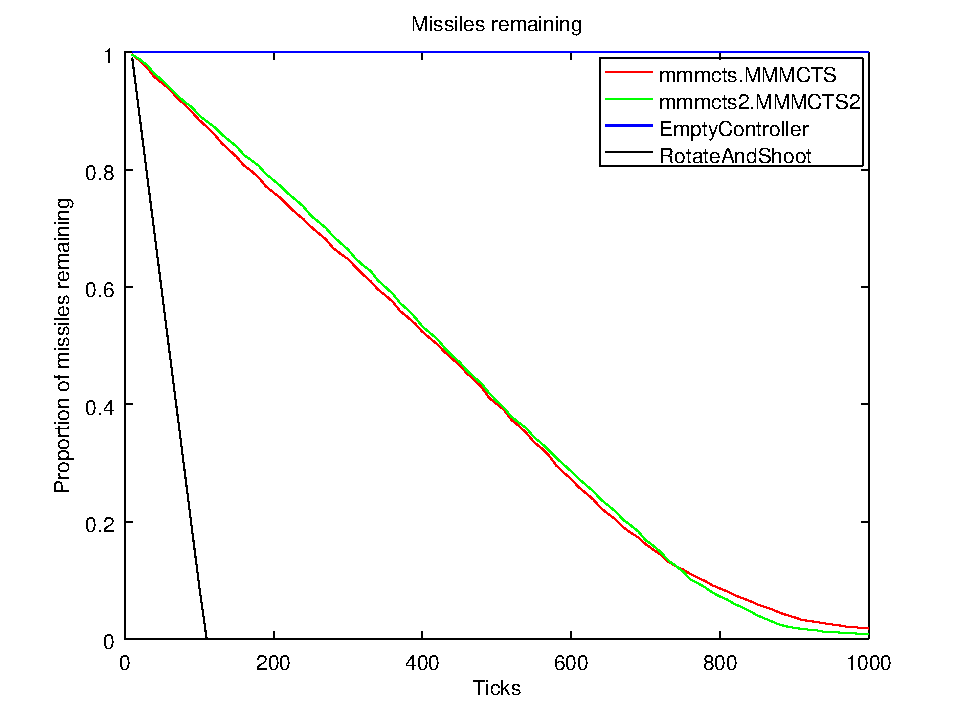
\includegraphics[scale=0.4]{resources/missiles_1.pdf}
\end{figure*}

\begin{figure*}
	\caption{Average metrics for AI players over the game with splitting asteroids}
	\label{fig:data3}
	\center
	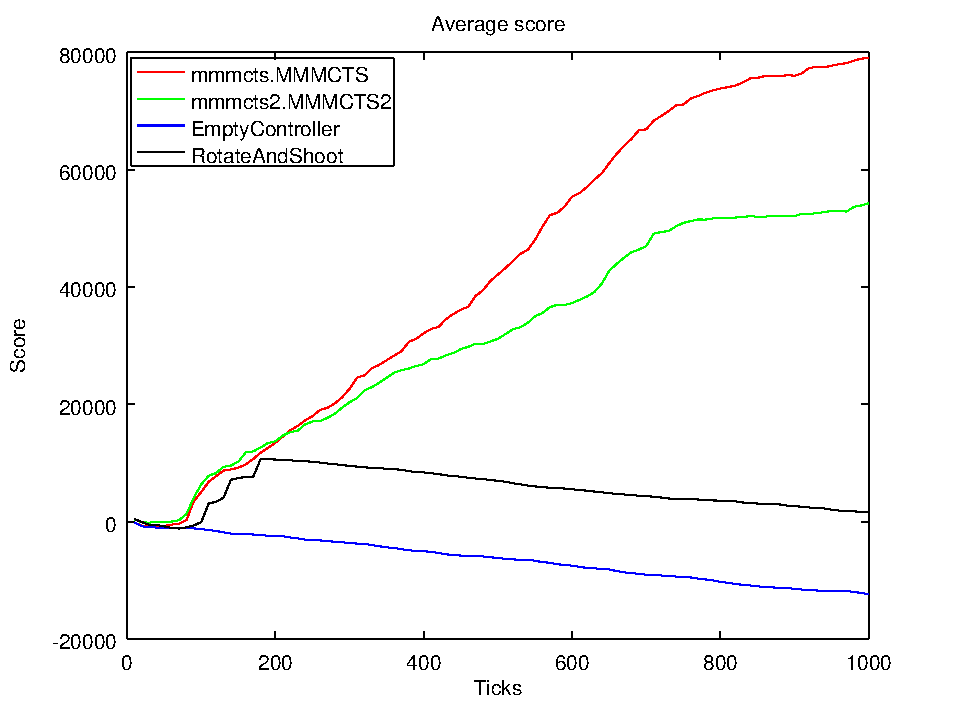
\includegraphics[scale=0.4]{resources/score_0.pdf}
	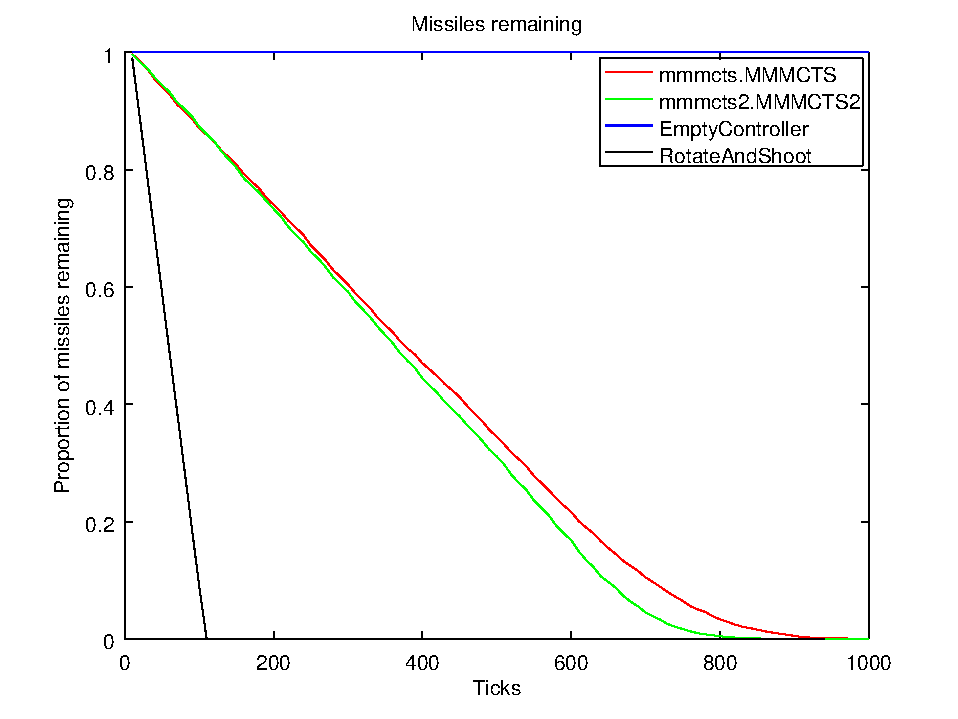
\includegraphics[scale=0.4]{resources/missiles_0.pdf}
\end{figure*}